\documentclass[9pt]{beamer}
\usepackage{minted}
%\usemintedstyle{manni}
\usemintedstyle{murphy}
\usepackage{hyperref}
\hypersetup{
colorlinks=true,
urlcolor=blue
}
\usepackage{graphicx}

\begin{document}
\title{Basic Introduction to gcloud}
\author{Nick Thompson} 
\date{\today}

\frame{\titlepage}

\begin{frame}[fragile]
  \frametitle{Goals of this discussion}
  \pause
  \begin{itemize}
  \item Learn how to rent CPUs and RAM from google
    \pause
  \item Learn how to rent persistent disks
    \pause
  \item Learn how to control expenses
    \pause
  \item Learn how to manage permissions
    \pause
  \item Learn how to create teams of identical VMs
    \pause
  \item Learn how to autoscale nodes based on load
  \end{itemize}
\end{frame}

\begin{frame}[fragile]
  \frametitle{What we won't discuss, but should}
  \pause
  \begin{itemize}
  \item The Python/Go/Node bindings
    \pause
  \item The REST (representational state transfer) interface
    \pause
  \item gcloud sql
    \pause
  \item Google Container Engine
    \pause
  \item Lots more . . .
  \end{itemize}
\end{frame}

\begin{frame}[fragile]
\frametitle{Getting started:}
\begin{minted}{bash}
$ curl https://sdk.cloud.google.com | bash
$ exec -l $SHELL
$ gcloud init
$ gcloud auth login
$ firefox https://console.developers.google.com
\end{minted}
You don't need a gmail account to use gcloud, but you must enter an email into gcloud that then becomes your google account login.
\end{frame}

\begin{frame}[fragile]
  \frametitle{Starting a Project}
  \begin{figure}
    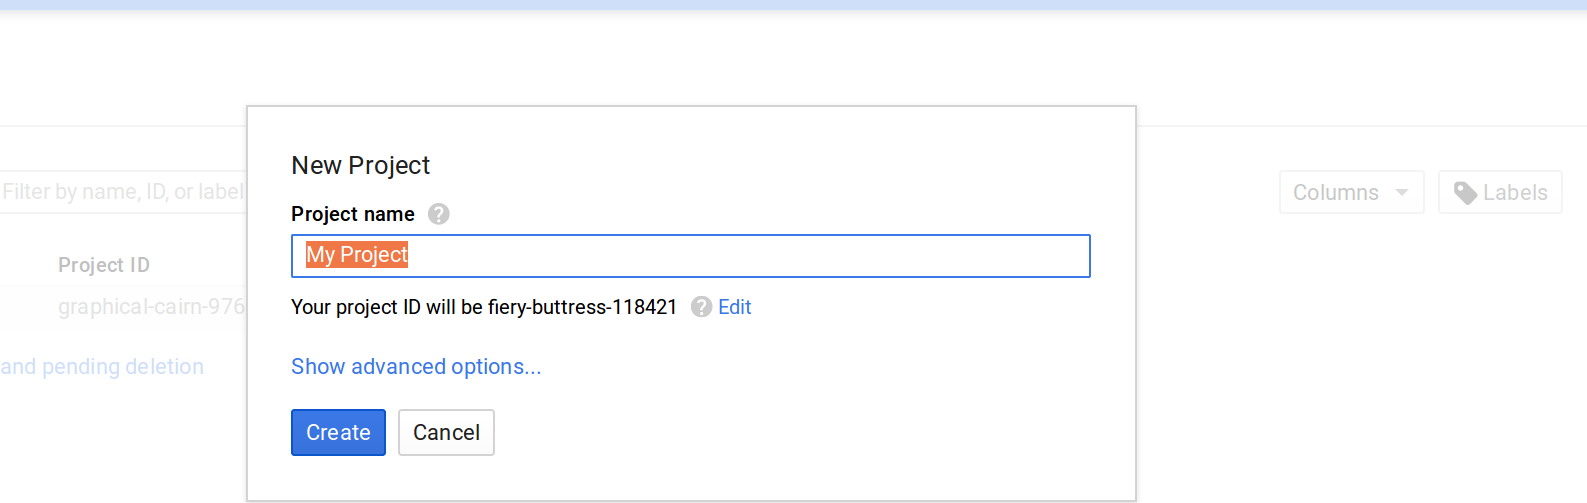
\includegraphics[scale=0.2]{figures/CreateProject.png}
  \end{figure}
\end{frame}

\begin{frame}[fragile]
  \frametitle{Starting a Project}
  Each project has
  \pause
  \begin{itemize}
  \item its bill separated in the invoice (1 billing account $\mapsto$ many project accounts)
    \pause
  \item its own VMs
    \pause
  \item its own persistent disks
    \pause
  \item its own users with their associated permissions.
  \end{itemize}
\end{frame}

\begin{frame}[fragile]
  \frametitle{Starting a Project}
  Multiple people can be listed as project owners, or given read access, or read/write access to the project:
  \begin{figure}
    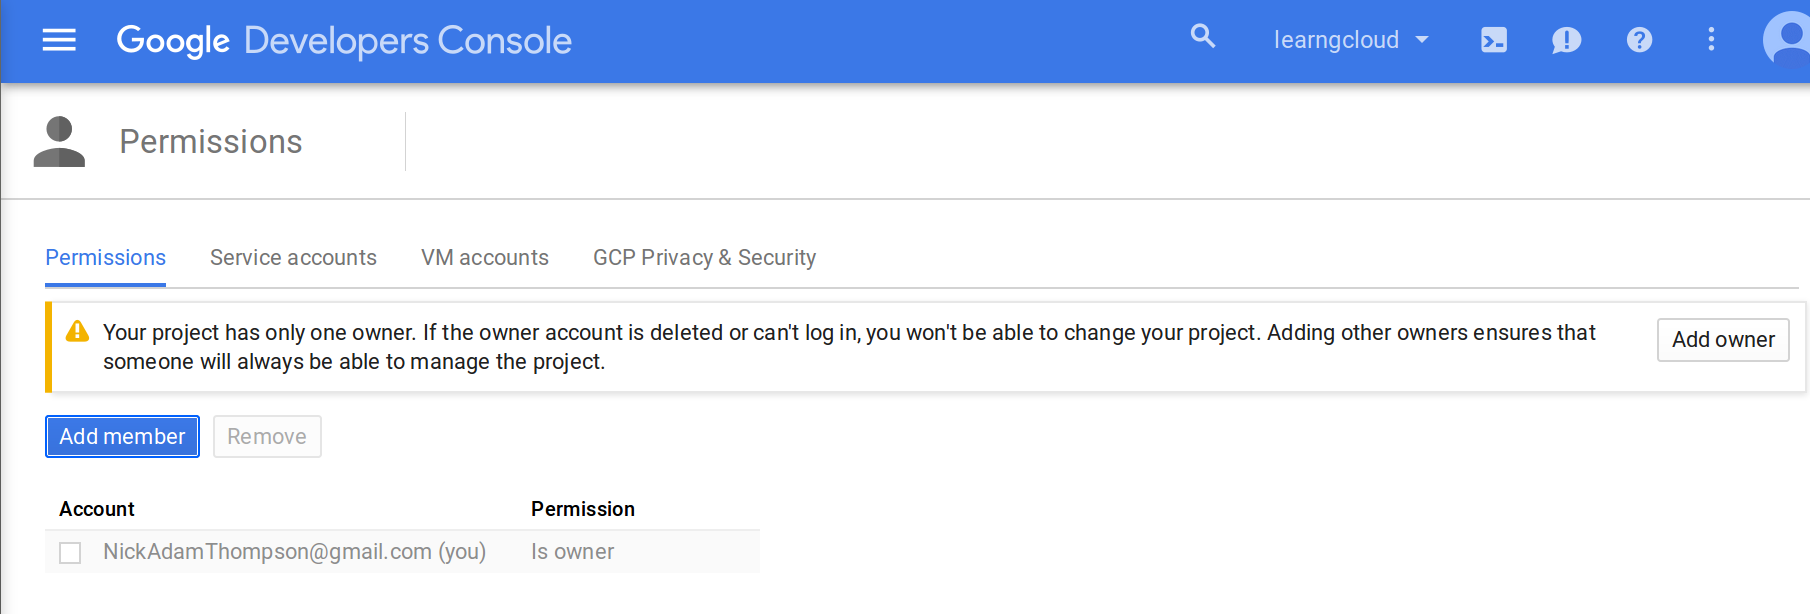
\includegraphics[scale=0.2]{figures/AddProjectOwner.png}
  \end{figure}
  \emph{Note that people who only have read access to the project nonetheless have root access to all the VMs!}
\end{frame}

\begin{frame}[fragile]
  \frametitle{Permissions}
The permission levels for a project are
\begin{itemize}
\pause
\item Owners-who can add/remove team members, and rent resources, and are root on resources
\pause	
\item Editors-who can rent resources, and are root on resources
\pause
\item Viewers-who can't rent resources, but are root on resources
\end{itemize}
\end{frame}


\begin{frame}[fragile]
  \frametitle{Starting a Project}
  When you grant someone permission to view/edit/co-own your project, they receive an email asking them if they want to join:
  \begin{figure}
    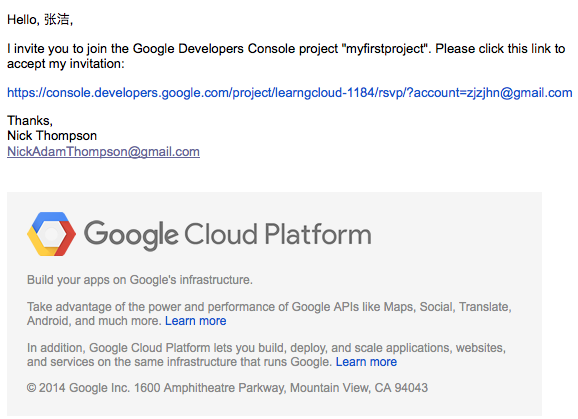
\includegraphics[scale=0.4]{figures/EmailConfirmation.png}
  \end{figure}
\end{frame}

\begin{frame}[fragile]
  \frametitle{gcloud user accounts}
  gcloud user accounts are in beta, and seem to be evolving rapidly. To see more, use
  \begin{minted}{bash}
$ gcloud beta compute users -h
  \end{minted}
or visit the \href{https://cloud.google.com/compute/docs/access/user-accounts/}{docs}.
\end{frame}

\begin{frame}[fragile]
  \frametitle{gcloud user accounts}
  Users with read-only access to your project have root on your VMs, but they can't launch new VMs on your dime:
  \begin{figure}
    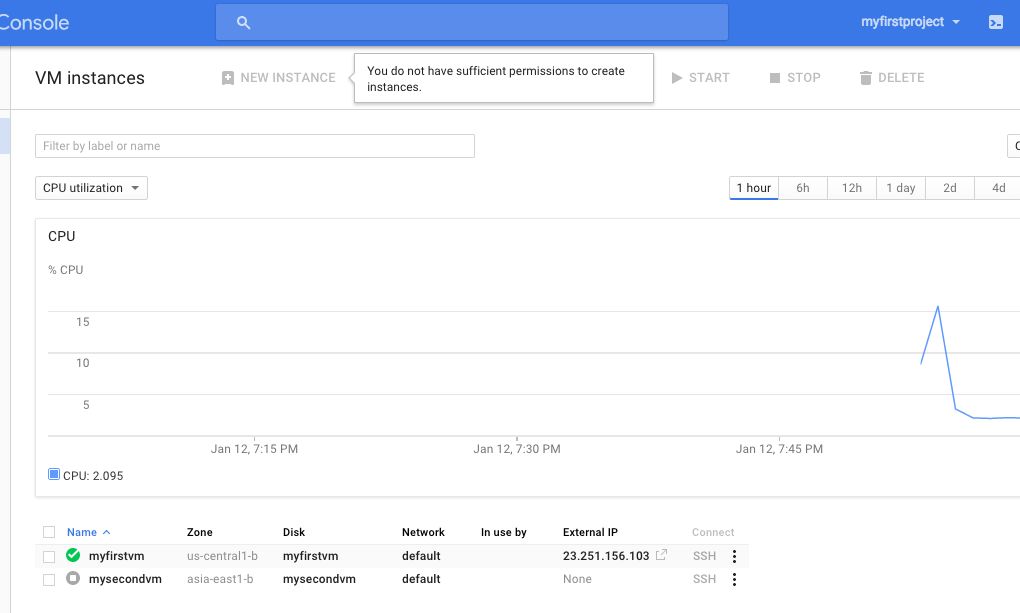
\includegraphics[scale=0.2]{figures/CantCreateVM.png}
  \end{figure}
\end{frame}


\begin{frame}[fragile]
\frametitle{Starting a project}
You need tell the gcloud command-line tool that you've created a new project:
\begin{minted}{bash}
$ gcloud config list
[core]
account = nickadamthompson@gmail.com
disable_usage_reporting = True
project = graphical-cairn-97618 
[meta]
active_config = default
\end{minted}
If the \texttt{project} field has the wrong value, you need to set it:
\begin{minted}{bash}
$ gcloud config set project learngcloud-1184
\end{minted}
Note that you don't set the project \emph{name}, you set the project \emph{ID}.
\end{frame}


\begin{frame}[fragile]
  \frametitle{Setting up an instance}
  \begin{figure}
    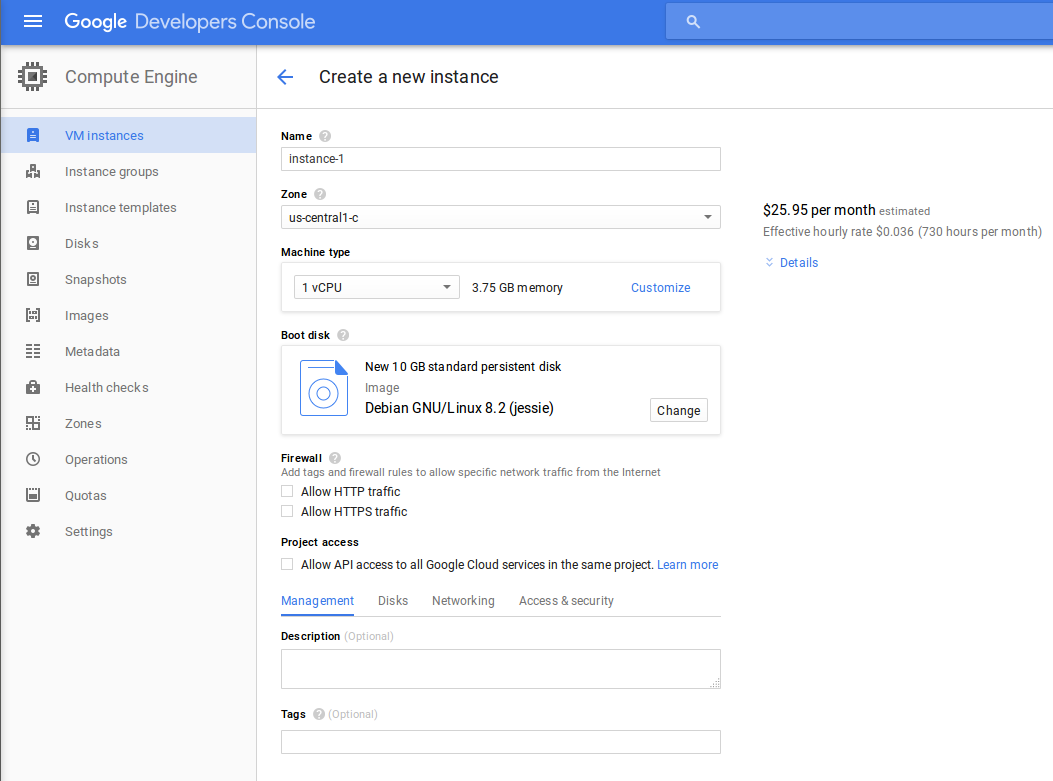
\includegraphics[scale=0.3]{figures/CreateInstance.png}
  \end{figure}
\end{frame}

\begin{frame}[fragile]
  \frametitle{Setting up an instance}
  Things to choose at this point:
  \pause
  \begin{itemize}
  \item Number of cores (min ~1/2, max 32)
    \pause
  \item amount of RAM (min 0.6GB, max unlimited, it seems, but 200GB is supported for sure)
    \pause
  \item size of disk, SSD (max 10TB) or spinning (max 10TB) 
    \pause
  \item Operating system (Ubuntu, Centos, CoreOS), or choose a VM snapshot
    \pause
  \item Firewall rules
    \pause
  \item Whether to use static or ephemeral IP addresses (static IPs cost money!)
  \end{itemize}
\end{frame}

\begin{frame}[fragile]
  \frametitle{Setting up an instance}
  Aside: If you need more than 10TB of disk space, you need to fill out the \href{https://docs.google.com/a/google.com/forms/d/1vb2MkAr9JcHrp6myQ3oTxCyBv2c7Iyc5wqIKqE3K4IE/viewform}{Google Compute Engine Quota Change Request Form}.
\end{frame}

\begin{frame}[fragile]
  \frametitle{Setting up an instance}
  Once you create a VM, you'll be assigned an external IP address and can see the load on your server:
  \begin{figure}
    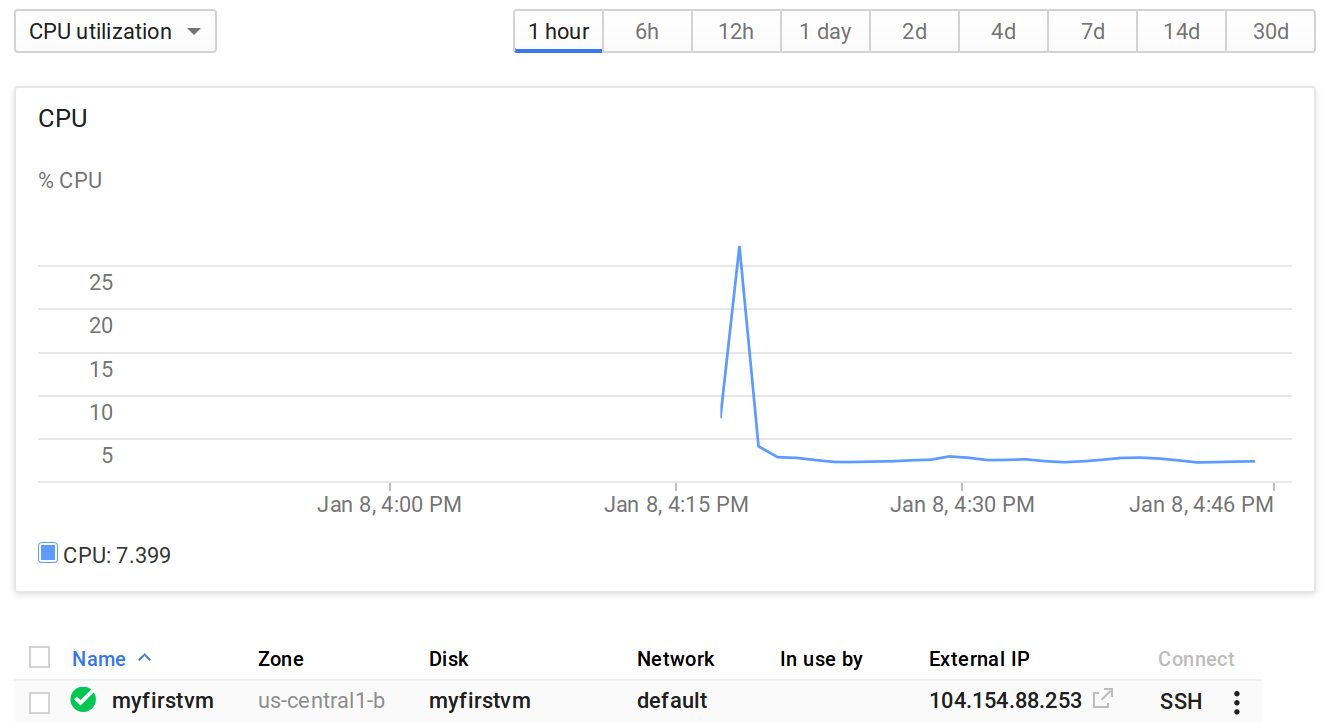
\includegraphics[scale=0.2]{figures/VMUp.png}
  \end{figure}
\end{frame}

\begin{frame}[fragile]
  \frametitle{Setting up an instance}
  To access your VM, use:
  \begin{minted}{bash}
    $ gcloud compute ssh myfirstvm --zone us-central1-b
  \end{minted}
  (Don't choose the wrong zone or else your instance won't be found!)

  This is really a wrapper script around the IP address of your instance:
  \begin{minted}{bash}
    $ ssh -i ~/.ssh/google_compute_engine 104.154.88.253
  \end{minted}
\end{frame}

\begin{frame}[fragile]
\frametitle{Setting up an instance}
For every console action, there is a equivalent gcloud command. So, for example, to set up an instance, you could type
\begin{minted}{bash}
$ gcloud compute instances create mysecondvm \
      --image ubuntu-15-10 --zone us-central1-b
\end{minted}
This is useful for scripting.
\end{frame}

\begin{frame}[fragile]
\frametitle{Exercise}
Why doesn't the following code work?
\begin{minted}{bash}
local$ gcloud compute instances create vm1 --zone us-central1-b
local$ gcloud compute ssh vm1
vm1$ gcloud compute instances create vm2 --zone us-central1-b
ERROR: (gcloud.compute.instances.create) Failed to find image for alias [debian-7-backports] in public image project [debian-cloud].
 - Insufficient Permission
\end{minted}
\end{frame}

\begin{frame}[fragile]
\frametitle{Solution}
\emph{You} are logged into gcloud, and can rent resources. However, your VM isn't you, and it doesn't have permission to rent resources on your behalf.

You can solve this problem by authorizing your VM to be able to rent resources using a \emph{service account}.
\end{frame}

\begin{frame}[fragile]
\frametitle{Service Accounts}
To authorize a VM to rent resources on your behalf, use the \emph{scopes} tag:
\begin{minted}{bash}
$ gcloud compute instances create vm-scoped \
    --scopes compute-rw --zone us-central1-b
\end{minted}
This gives your vm permission to spawn new vms.
\end{frame}

\begin{frame}[fragile]
  \frametitle{Startup Scripts}
  To get an image configured for autoscaling, we need to specify what sort of software we need on the image before it's creation. We can do this via a ``startup script'':
  \begin{figure}
    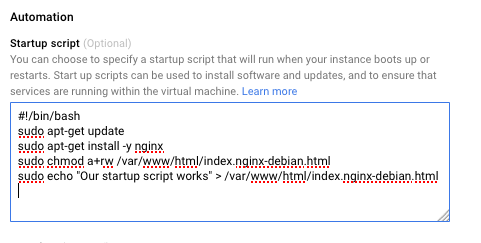
\includegraphics[scale=0.5]{figures/StartupScript.png}
  \end{figure}
\end{frame}

\begin{frame}[fragile]
	\frametitle{Startup Scripts}
	It works!
	\begin{minted}{bash}
	$ curl 130.211.135.33
	Our startup script works
	\end{minted}
	However, this is not a good design; as the startup script is not in source control.
\end{frame}

\begin{frame}[fragile]
\frametitle{Startup Scripts}
Once your startup script is in source control, you can easily deploy a new instance via:
\begin{minted}{bash}
$ gcloud compute instances create wstartup \
   --metadata-from-file startup-script=script.sh \
   --zone=us-central1-b  --tags "http-server"
Created [https://www.googleapis.com/compute/v1/projects/learngcloud-1184/zones/us-central1-a/instances/wstartup].
NAME     ZONE          MACHINE_TYPE  PREEMPTIBLE INTERNAL_IP EXTERNAL_IP    STATUS
wstartup us-central1-a n1-standard-1             10.240.0.5  104.197.59.116 RUNNING
$ curl 104.197.59.116
Our startup script works
\end{minted}
\end{frame}

\begin{frame}[fragile]
\frametitle{Startup Scripts}
Note that you can ssh into your machine before the startup script has finished! To see if your startup script has finished, or to debug your startup script:
\begin{minted}{bash}
$ gcloud compute ssh wstartup --zone=us-central1-b
wstartup$ cat /var/log/startupscript.log
...
ubuntu startupscript: Finished running startup script /var/run/google.startup.script
\end{minted}
\end{frame}

\begin{frame}[fragile]
\frametitle{Regions and Zones}
Google divides the world into regions:
\begin{minted}{bash}
$ gcloud compute regions list
NAME         CPUS          DISKS_GB     ADDRESSES RESERVED_ADDRESSES STATUS TURNDOWN_DATE
asia-east1      0.00/24.00     10/10240      0/23      0/7           UP
europe-west1    0.00/24.00      0/10240      0/23      0/7           UP
us-central1     4.00/24.00     40/10240      4/23      0/7           UP
us-east1        0.00/24.00      0/10240      0/23      0/7           UP
\end{minted}
\end{frame}

\begin{frame}[fragile]
\frametitle{Regions and Zones}
And each region is divided into multiple zones
\begin{minted}{bash}
$ gcloud compute zones list
NAME           REGION       STATUS NEXT_MAINTENANCE TURNDOWN_DATE
asia-east1-a   asia-east1   UP
asia-east1-b   asia-east1   UP
asia-east1-c   asia-east1   UP
europe-west1-b europe-west1 UP
europe-west1-d europe-west1 UP
europe-west1-c europe-west1 UP
us-central1-c  us-central1  UP
us-central1-a  us-central1  UP
us-central1-f  us-central1  UP
us-central1-b  us-central1  UP
us-east1-c     us-east1     UP
us-east1-b     us-east1     UP
us-east1-d     us-east1     UP
\end{minted}
\end{frame}

\begin{frame}[fragile]
\frametitle{Regions and Zones}
A zone is essentially single datacenter, so two instances in a zone can communicate very quickly with one another:
\begin{minted}{bash}
vmcentral1b-1$ ping vmcentral1b-2 # ping VM in same datacenter/zone:
rtt min/avg/max/mdev = 0.308/0.394/0.841/0.104 ms
vmcentral1b-1$ ping vmcentral1a # Ping VM in same region, different zone:
rtt min/avg/max/mdev = 0.571/0.673/1.210/0.099 ms
vmcentral1b-1$ ping vm-in-asia 
rtt min/avg/max/mdev = 154.738/154.878/155.326/0.442 ms
\end{minted}
 So within-zone communication is fastest, within-region is fast, between-region is slow. (Note how your instance names are resolved via DNS!)
\end{frame}

\begin{frame}[fragile]
\frametitle{Regions and Zones}
Things you rent from Google are classified by their scope in the global/regional/zonal hierarchy. For instance,
\begin{itemize}
\pause
\item Images, VM snapshots, firewall rules, and buckets are global resources
\pause
\item Addresses are regional resources
\pause
\item Instances and their boot disks are zonal resources
\end{itemize}
\end{frame}

\begin{frame}[fragile]
\frametitle{Exercise}
Why does google need to ask us for the zone for almost every command?
\begin{minted}{bash}
$ gcloud compute instances describe vm2
For the following instances:
 - [vm2]
choose a zone:
 [1] asia-east1-a
 ...
\end{minted}
\end{frame}

\begin{frame}[fragile]
\frametitle{Solution}
Everything action in gcloud is achieved via REST (representational state transfer).

This is a POST/GET/DELETE/PUT request to an html endpoint, and the endpoint url contains the zone!
\begin{figure}
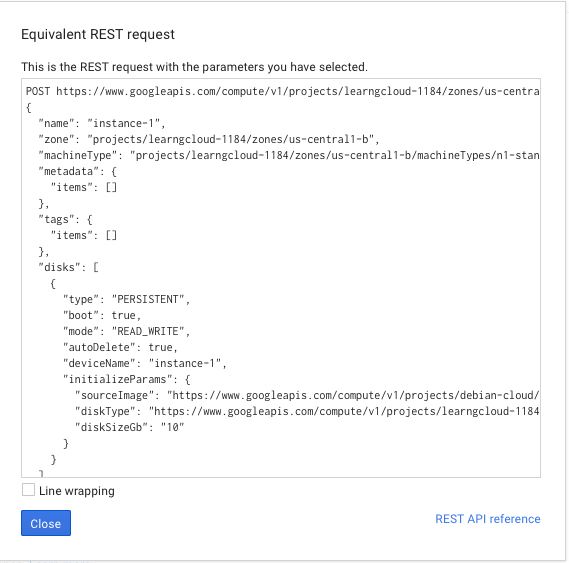
\includegraphics[scale=0.3]{figures/EquivalentRest.png}
\end{figure}
\end{frame}

\begin{frame}[fragile]
\frametitle{Snapshotting an instance}
  Once you have installed your favorite software on your VM, you might want to snapshot it:
  \begin{minted}{bash}
myfirstvm$ sudo apt-get update
myfirstvm$ sudo apt-get install -y gcc g++ emacs git
myfirstvm$ sudo touch /opt/hello.txt && sudo chmod a+rw /opt/hello.txt
myfirstvm$ echo "Hello from GCE!" >> /opt/hello.txt
myfirstvm$ exit
localhost$ gcloud compute disks snapshot "myfirstvm" \
              --zone "us-central1-b" --snapshot-names "firstvmsnapshot"
  \end{minted}  
\end{frame}

\begin{frame}[fragile]
  \frametitle{Snapshotting an instance}
  Of course, using the console GUI is a bit easier:
  \begin{figure}
    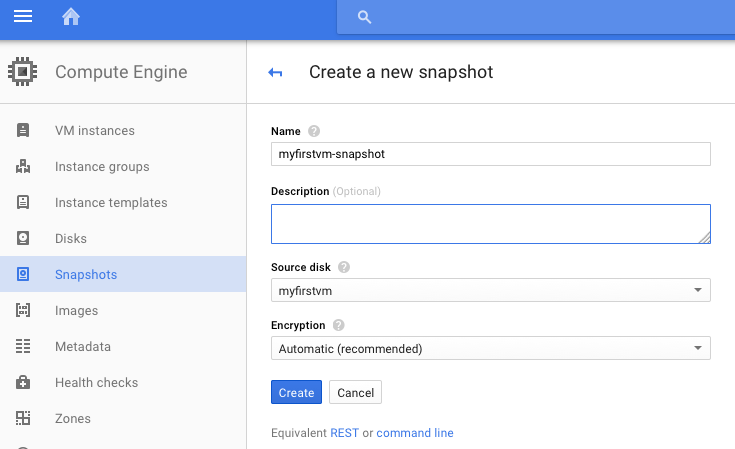
\includegraphics[scale=0.3]{figures/SnapshotVM.png}
  \end{figure}
\end{frame}

\begin{frame}[fragile]
  \frametitle{Snapshotting an instance}
  Once you have a snapshot, you can create a boot disk from it:
\begin{figure}
  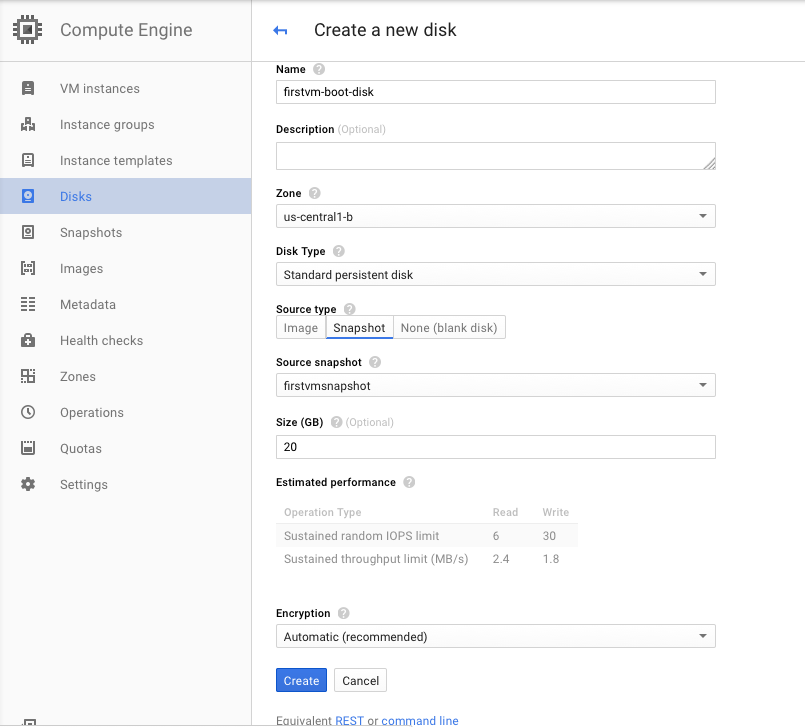
\includegraphics[scale=0.3]{figures/BootDisk.png}
\end{figure}
\end{frame}

\begin{frame}[fragile]
  \frametitle{Snapshotting an instance}
  And once you have a boot disk, you can create a VM from it:
  \begin{figure}
    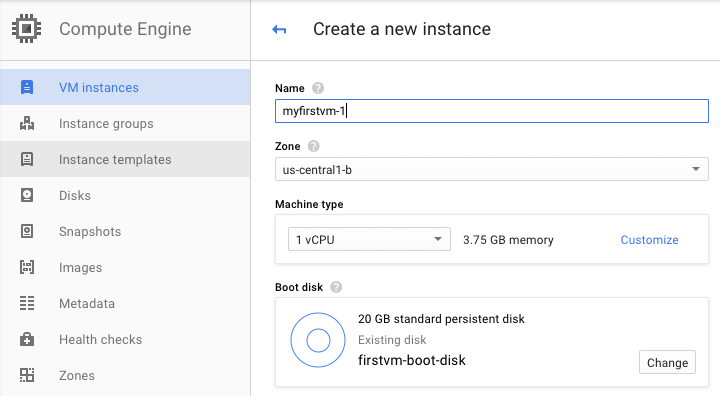
\includegraphics[scale=0.3]{figures/VMFromBootDisk.png}
  \end{figure}
\end{frame}

\begin{frame}[fragile]
  \frametitle{Replicating VMs}
  A boot disk can only be attached in RW mode to a single instance. To attach a boot disk in read-only mode to many instances, use
  \begin{minted}{bash}
$ gcloud compute instances create vm-{1..3} --zone us-central1-b \
   --disk name=firstvm-boot-disk,boot=yes,mode=ro
  \end{minted}
A read-only boot disk is a pain! This is how we get identical snapshots with read/write boot disks:
\begin{minted}{bash}
$ gcloud compute disks create vm-{1..5}  \
    --source-snapshot "vm-snapshot"  --zone us-central1-b
$ for i in {1..5}; do gcloud compute instances create vm-$i \
    --zone=us-central1-b --disk name=vm-$i,mode=rw,boot=yes; done
\end{minted}
\end{frame}

\begin{frame}[fragile]
\frametitle{Exercise}
You created an n1-standard-1 VM to serve a website. However, since this VM is handling the load with very little CPU usage, you realize you can save money by using a shared-CPU instance.

Exercise: Use persistent boot disks to migrate your server from an n1-standard-1 instance to an f1-micro instance.
\end{frame}

\begin{frame}[fragile]
\frametitle{Exercise}
Step 1: Create the standard instance:
\begin{minted}{bash}
$ gcloud compute instances create myserver \
    --zone=us-central1-b --machine-type=n1-standard-1 \
    --tags=http-server
Created [https://www.googleapis.com/compute/v1/projects/learngcloud-1184/zones/us-central1-b/instances/myserver].
NAME     ZONE          MACHINE_TYPE  PREEMPTIBLE INTERNAL_IP EXTERNAL_IP     STATUS
myserver us-central1-b n1-standard-1             10.240.0.3  130.211.120.111 RUNNING
\end{minted}
\end{frame}

\begin{frame}[fragile]
\frametitle{Exercise}
Step 2: Start an nginx-server on this instance:
\begin{minted}{bash}
$ gcloud compute ssh myserver --zone=us-central1-b
myserver$ sudo apt-get update && sudo apt-get install -y nginx
myserver$ sudo chmod a+rw /var/www/html/index.nginx-debian.html
myserver$ echo "Hola!" > /var/www/html/index.nginx-debian.html
myserver$ exit
$ curl 130.211.120.11 # Make sure it works!
Hola!
\end{minted}
\end{frame}

\begin{frame}[fragile]
\frametitle{Exercise}
Step 3: Delete your instance, but keep the boot disk!
\begin{minted}{bash}
$ gcloud compute instances delete myserver \
   --keep-disks boot --zone=us-central1-b
 $ gcloud compute disks list
NAME              ZONE          SIZE_GB TYPE        STATUS
myserver          us-central1-b 10      pd-standard READY
\end{minted}

\end{frame}

\begin{frame}[fragile]
\frametitle{Exercise}
Step 4: Create a new instance from the boot disk:
\begin{minted}{bash}
$ gcloud compute instances create smaller-server \
--zone=us-central1-b --machine-type=f1-micro \
    --tags=http-server --disk name=myserver,boot=yes,mode=rw
Created [https://www.googleapis.com/compute/v1/projects/learngcloud-1184/zones/us-central1-b/instances/smaller-server].
NAME           ZONE          MACHINE_TYPE INTERNAL_IP EXTERNAL_IP     STATUS
smaller-server us-central1-b f1-micro     10.240.0.3  130.211.120.111 RUNNING
$ curl 130.211.120.111
Hola!
\end{minted}
\end{frame}

\begin{frame}[fragile]
  \frametitle{Editing Firewalls}
  Google cloud has a set of default firewall rules that you might like to edit:
  \begin{figure}
    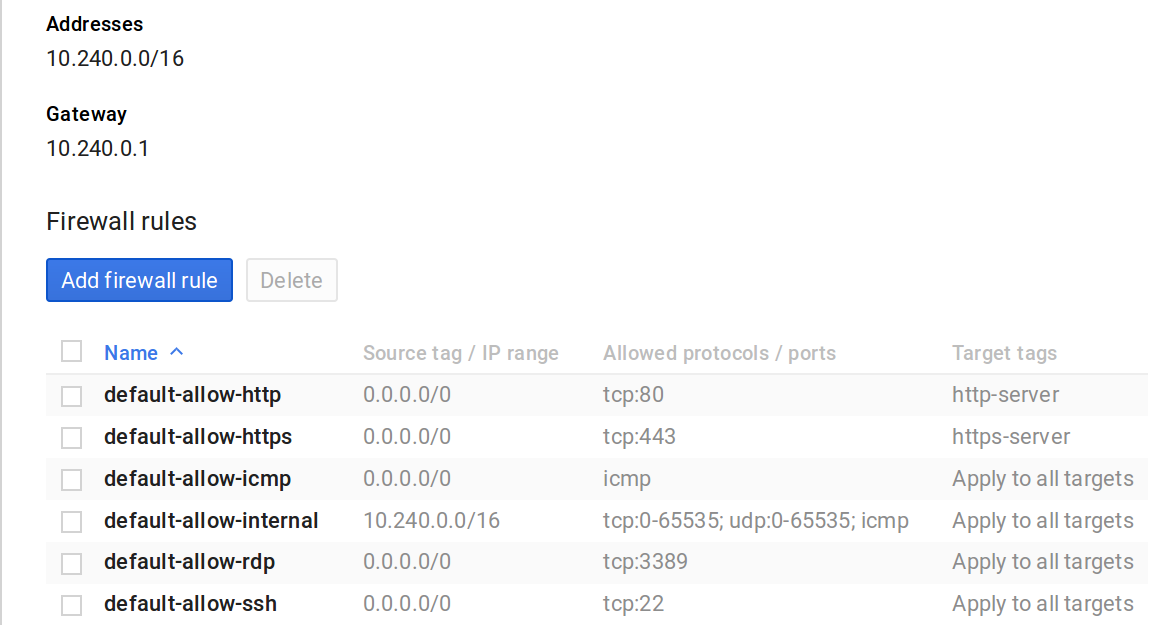
\includegraphics[scale=0.2]{figures/DefaultFirewall.png}
  \end{figure}
\end{frame}

\begin{frame}[fragile]
Note that all ports are available via the internal ip addresses 10.240.0.0/16
  \begin{minted}{bash}
$ gcloud compute firewall-rules list
NAME                   NETWORK SRC_RANGES    RULES                        SRC_TAGS TARGET_TAGS
default-allow-http     default 0.0.0.0/0     tcp:80                                http-server
default-allow-https    default 0.0.0.0/0     tcp:443                               https-server
default-allow-icmp     default 0.0.0.0/0     icmp
default-allow-internal default 10.240.0.0/16 tcp:0-65535,udp:0-65535,icmp
default-allow-ssh      default 0.0.0.0/0     tcp:22    
  \end{minted}

\end{frame}

\begin{frame}[fragile]
  \frametitle{Editing Firewalls}
  The default rules are of course reflected in the port scan:
  \begin{minted}{bash}
    $ nmap -p 0-10000 104.154.88.253

    Starting Nmap 6.47 ( http://nmap.org ) at 2016-01-08 17:43 CST
    Nmap scan report for 253.88.154.104.bc.googleusercontent.com (104.154.88.253)
    Host is up (0.040s latency).
    Not shown: 9997 filtered ports
    PORT     STATE  SERVICE
    22/tcp   open   ssh
    80/tcp   closed http
    443/tcp  closed https
    3389/tcp closed ms-wbt-server
  \end{minted}
\end{frame}

\begin{frame}[fragile]
  \frametitle{Editing firewalls}
  This allows traffic from AMQP:
  \begin{figure}
    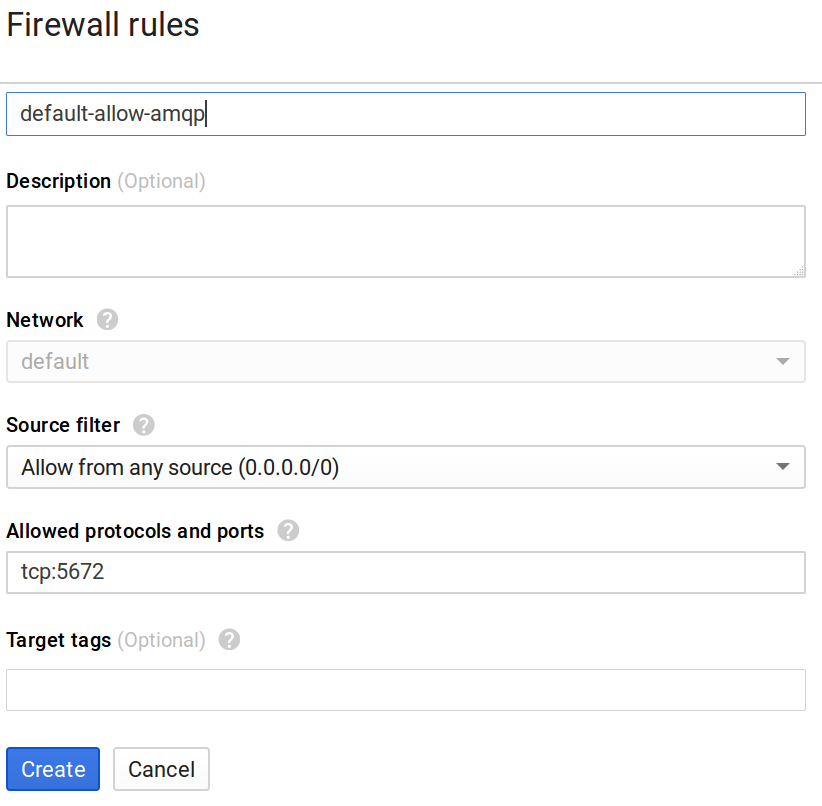
\includegraphics[scale=0.2]{figures/DefineFirewall.png}
  \end{figure}
\end{frame}

\begin{frame}[fragile]
  \frametitle{Editing firewalls}
  Command line to allow AMQP on port 5672 from any source IP, use the command
\begin{minted}{bash}
$ gcloud compute firewall-rules \ 
   create default-allow-amqp --allow tcp:5672 \
   --target-tags rabbit-server
Created [https://www.googleapis.com/compute/v1/projects/learngcloud-1184/global/firewalls/default-allow-amqp].
NAME               NETWORK SRC_RANGES RULES    SRC_TAGS TARGET_TAGS
default-allow-amqp default 0.0.0.0/0  tcp:5672					  rabbit-server
\end{minted}
Creating a firewall rule applies it to all live instances in the project, unless you give it a target-tag.
\end{frame}

\begin{frame}[fragile]
\frametitle{Target Tags}
Target tags give us an idea of what our instance is going to be used for. This tag allows traffic on port 80/443:
\begin{minted}{bash}
$ gcloud compute instances create webserver \
 --zone us-central1-b --tags http-server,https-server
\end{minted}
Our custom amqp firewall rule will be applied to this server:
\begin{minted}{bash}
$ gcloud compute instanes create rabbit \
--zone us-central1-b --tags rabbit-server
\end{minted}
\end{frame}

\begin{frame}[fragile]
  \frametitle{Networking}
  Each project supports a $2^{16} = 65,536$ address internal network:
  \begin{minted}{bash}
$ gcloud compute networks list
NAME    IPV4_RANGE    GATEWAY_IPV4
default 10.240.0.0/16 10.240.0.1    
  \end{minted}
\end{frame}

\begin{frame}[fragile]
\frametitle{Load balancing}
Let's set up a couple servers to learn how to load balance. First, our startup script.sh:
\begin{minted}{bash}
#!/bin/bash
sudo apt-get update
sudo apt-get install -y nginx emacs
sudo chmod a+rw /var/www/html/index.nginx-debian.html 
sudo echo "Hello from $(hostname)" > /var/www/html/index.nginx-debian.html
\end{minted}  
\end{frame}

\begin{frame}[fragile]
\frametitle{Load balancing}
Now create your servers with this startup script:
 \begin{minted}{bash}
$ gcloud compute instances create server-{1..3} \
    --tags http-server --zone us-central1-a \
    --metadata-from-file startup-script=script.sh
  \end{minted}
\end{frame}

\begin{frame}[fragile]
\frametitle{Load Balancing}
Now let's set up a ``target-pool'', a group of server that responds to requests:
\begin{minted}{bash}
$ gcloud compute target-pools create \
    mypool --region us-central1
$ gcloud compute target-pools add-instances \ 
    mypool --instances server-{1..3} --zone us-central1-a
$ gcloud compute forwarding-rules create \
  frontend-forwarding --target-pool mypool --region us-central1
NAME      REGION      IP_ADDRESS     IP_PROTOCOL TARGET
frontends us-central1 104.154.36.151 TCP         us-central1/targetPools/frontends
$ for i in {1..100}; do curl 104.154.36.151; done
Welcome to server-1!
Welcome to server-1!
Welcome to server-3!
Welcome to server-2!
Welcome to server-1!
\end{minted}
\end{frame}

\begin{frame}[fragile]
  \frametitle{Load Balancing}
  What happens if one of our servers stops?
\begin{minted}{bash}
$ for i in {1..100}; do curl 104.154.44.41; done
Hello from server-1!
Hello from server-3!
curl: (7) Failed to connect to 104.154.44.41 port 80: Connection refused
\end{minted}
The load balancer doesn't know anything about our servers, so it can't tell if it should send traffic there or not. Let's educate our load balancer:
\end{frame}

\begin{frame}[fragile]
\frametitle{Educating your load balancer}
We need our load balancer to know that the server on port 80 should be available. Therefore, we create a health-check for it:
\begin{minted}{bash}
$ gcloud compute http-health-checks create frontend-check
Created [https://www.googleapis.com/compute/v1/projects/learngcloud-1184/global/httpHealthChecks/frontend-check].
NAME           HOST PORT REQUEST_PATH
frontend-check      80   /
$ gcloud compute target-pools add-health-checks mypool \
   --http-health-check frontend-check --region=us-central1
Updated [https://www.googleapis.com/compute/v1/projects/learngcloud-1184/regions/us-central1/targetPools/frontend-targetpool].
\end{minted}
\end{frame}

\begin{frame}[fragile]
\frametitle{Load Balancer with Health Checks}
Now we shouldn't see many failed requests:
\begin{minted}{bash}
$ for i in {1..100}; do curl 104.154.44.41; done
Hello from server-1!
Hello from server-3!
Hello from server-1!
Hello from server-1!
Hello from server-3!
Hello from server-3!
Hello from server-3!
Hello from server-1!
Hello from server-3!
Hello from server-1!
Hello from server-3!
Hello from server-1!
Hello from server-1!
Hello from server-3!
Hello from server-3!
\end{minted}
\end{frame}

\begin{frame}[fragile]
\frametitle{Educating your load balancer}
For those who don't like the command line, of course we can create the health check in the console:
\begin{figure}[fragile]
    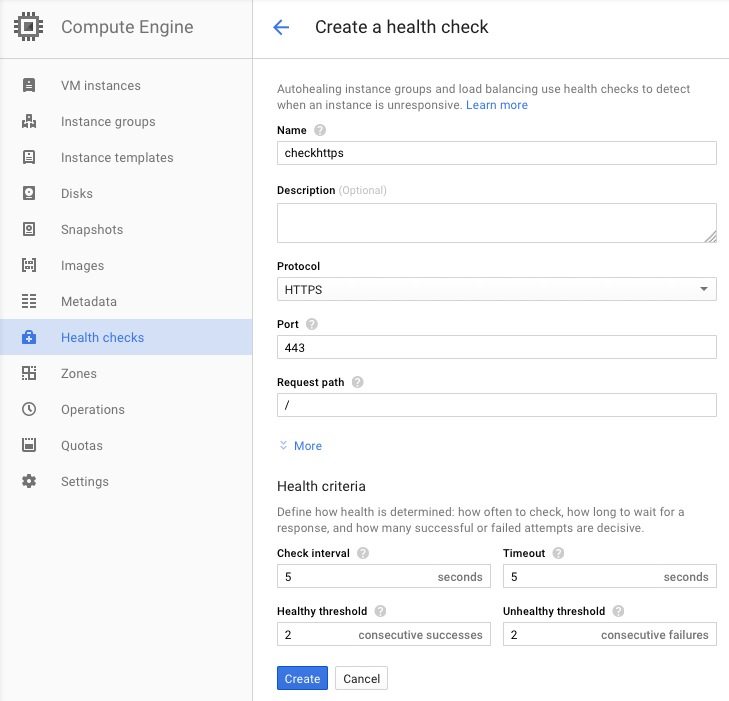
\includegraphics[scale=0.3]{figures/HealthCheck.png}
\end{figure}
\end{frame}

\begin{frame}[fragile]
  \frametitle{Instance Templates}
  Before autoscaling, we need to create an \emph{instance template}, which describes how big we want our nodes, what OS, and perhaps a startup script.
  
  Remember, these nodes must be identical.
  \begin{figure}
    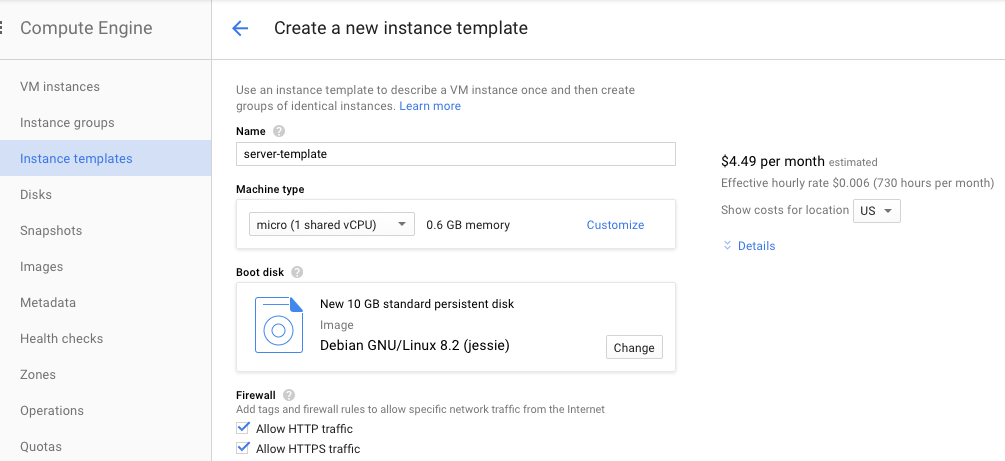
\includegraphics[scale=0.3]{figures/InstanceTemplate.png}
  \end{figure}
  You can also use a custom image instead of an instance template; this is preferred for complex deployments.
\end{frame}

\begin{frame}[fragile]
\frametitle{Instance Templates}
To create the instance template from the command line using a startup script, use:
\begin{minted}{bash}
$ gcloud compute instance-templates create my-instance-template \
  --machine-type=f1-micro --scopes=compute-rw,storage-full \
   --tags=http-server \
    --metadata-from-file startup-script=server_startup.sh
\end{minted}
Question 1: Why didn't we need to specify a zone here?

Question 2: Why do we need to tag this with ``http-server''?
\end{frame}

\begin{frame}[fragile]
\frametitle{Instance Groups}
Once we have an instance template, we can create an autoscaling instance group:
\begin{figure}
    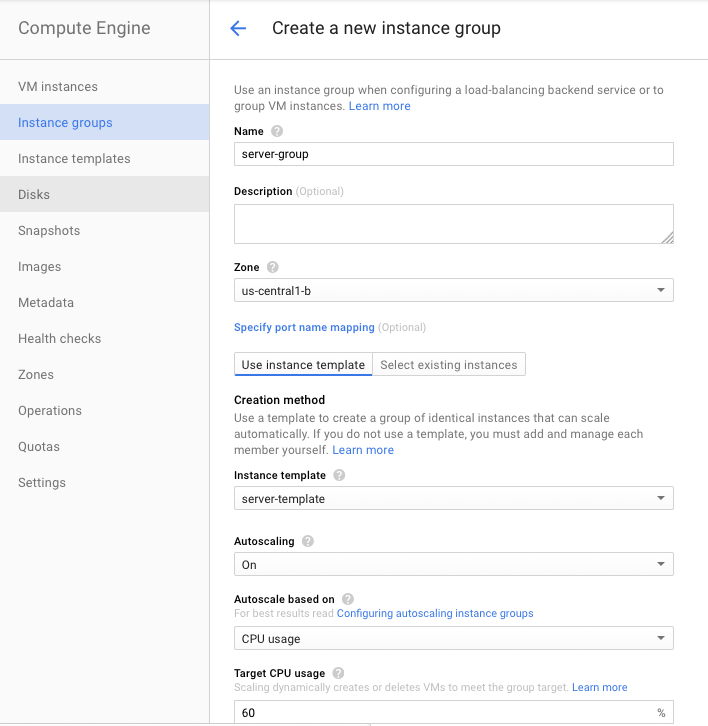
\includegraphics[scale=0.2]{figures/Autoscale.png}
\end{figure}
\end{frame}

\begin{frame}[fragile]
\frametitle{Instance Groups}
Command-line for creating instance groups:
\begin{minted}{bash}
$  gcloud compute instance-groups managed create my-instance-group \
   --zone us-central1-b --template my-instance-template \
    --base-instance-name my-instance-group --size 1
\end{minted}
\end{frame}

\begin{frame}[fragile]
\frametitle{Autoscaling an Instance Group}
Command line:
\begin{minted}{bash}
$ gcloud compute instance-groups managed set-autoscaling "my-instance-group" \
    --zone "us-central1-b" --cool-down-period "60" \
    --max-num-replicas "4" --min-num-replicas "1" \
    --target-cpu-utilization "0.6"
\end{minted}
This should now start autoscaling based on load!

\end{frame}

\begin{frame}[fragile]
\frametitle{Zonal Data Disks}
In addition to creation of boot disks, you can create zonal data disks:
\begin{minted}{bash}
$ gcloud compute disks create "data-disk" \
   --size=200 --zone=us-central1-b
Created [https://www.googleapis.com/compute/v1/projects/learngcloud-1184/zones/us-central1-b/disks/data-disk].
NAME      ZONE          SIZE_GB TYPE        STATUS
data-disk us-central1-b 200     pd-standard READY
\end{minted}
\end{frame}

\begin{frame}[fragile]
\frametitle{Zonal Data Disks}
We can now mount this on an instance:
\begin{minted}{bash}
$ gcloud compute instances create datavm \
   --scopes=compute-rw --zone=us-central1-b
$ gcloud compute ssh datavm --zone=us-central1-b
datavm$ gcloud compute instances attach-disk datavm --disk data-disk --zone=us-central1-b
datavm$ sudo mkdir -p /mnt/pd0
datavm$ ls -l /dev/disk/by-id/google*	
datavm$ sudo /usr/share/google/safe_format_and_mount -m "mkfs.ext4 -F" \
              /dev/disk/by-id/google-persistent-disk-1 /mnt/pd0
datavm$ df -k
...
\end{minted}
\end{frame}



\begin{frame}[fragile]
  \frametitle{Persistent Disks}
  If you need storage that is not chained to a particular zone, then you need to use ``buckets'':
  \begin{figure}
    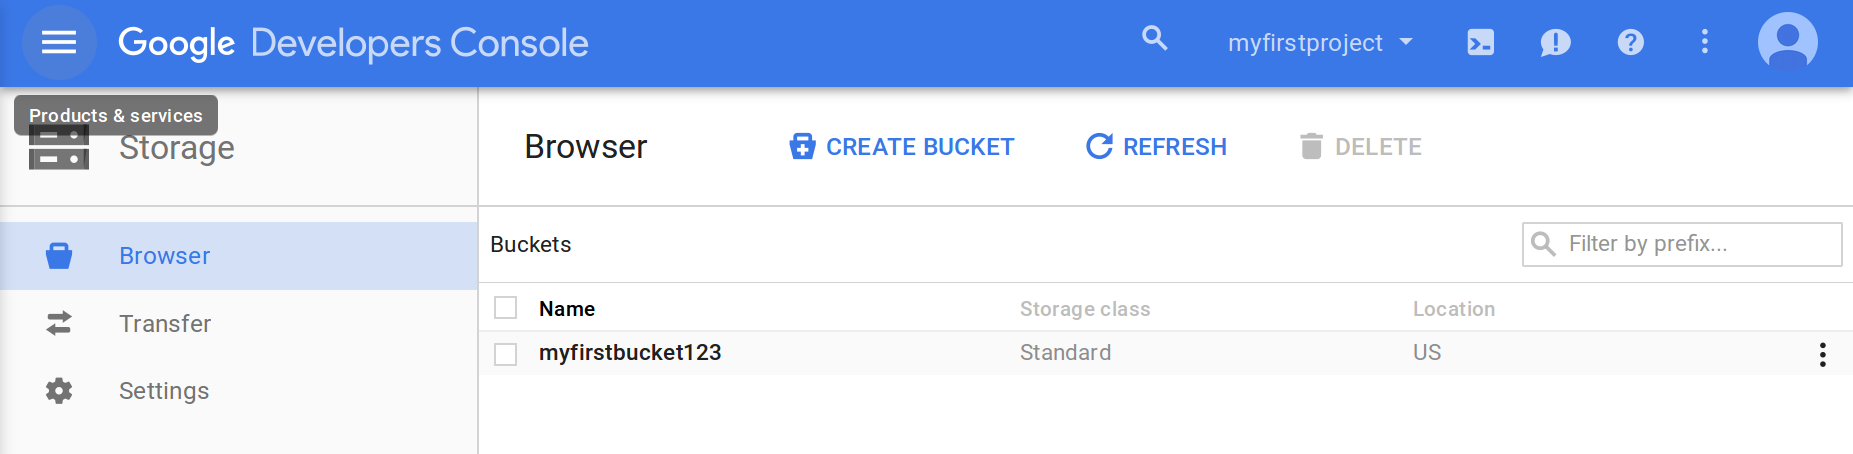
\includegraphics[scale=0.2]{figures/Buckets.png}
  \end{figure}
\end{frame}

\begin{frame}[fragile]
  \frametitle{Persistent Disks}
  In order to manage persistent disks from the command line, use the gsutil utility:
  \begin{minted}{bash}
    $ pip install gsutil
    $ gsutil mb gs://myfirstbucket
    Creating gs://myfirstbucket/...
    ServiceException: 409 Bucket myfirstbucket already exists.
    $ gsutil mb gs://myfirstbucket123
    Creating gs://myfirstbucket123/...
    $ gsutil cp talk.log gs://myfirstbucket123
    Copying file://talk.log [Content-Type=application/octet-stream]...
    Uploading   gs://myfirstbucket123/talk.log:                      43.94 KiB/43.94 KiB
    ~/learn_gcloud$ gsutil ls
    gs://myfirstbucket123/
    $ gsutil ls -l gs://myfirstbucket123
    44993  2016-01-09T21:19:30Z  gs://myfirstbucket123/talk.log
    TOTAL: 1 objects, 44993 bytes (43.94 KiB)
  \end{minted}
  Bucket names need to be globally unique across all of gcloud!
\end{frame}

\begin{frame}[fragile]
  \frametitle{Persistent Disks}
  \begin{itemize}
  \item gcloud buckets are encrypted on disk
  \item gcloud buckets are accessible outside zones (i.e. have global scope)
  \item Uploads to gcloud buckets are atomic and considered successful once the info is stored in multiple datacenters.
  \end{itemize}
\end{frame}

\begin{frame}[fragile]
\frametitle{Persistent Disks}
Mounting a bucket to an instance takes a little work (\href{https://github.com/googlecloudplatform/gcsfuse/blob/master/docs/installing.md}{instructions}). First let's create a startup script called can-bucket.sh:
\begin{minted}{bash}
#!/bin/bash
sudo apt-get update
sudo apt-get install -y fuse emacs
sudo curl -L -O \
https://github.com/GoogleCloudPlatform/gcsfuse/releases/download/v0.15.0/gcsfuse_0.15.0_amd64.deb
sudo dpkg --install gcsfuse_0.15.0_amd64.deb
\end{minted}
\end{frame}
\begin{frame}[fragile]
\frametitle{Persistent Disks}
Now let's create some instances which have permission to view our bucket:
\begin{minted}{bash}
$ gcloud compute instances create can-bucket-{1..3} \
   --zone=us-central1-b --scopes=storage-full \
   --metadata-from-file startup-script=can-bucket.sh
\end{minted}
The ``scopes=storage-full'' gives our instances permission to mount our buckets.
\end{frame}

\begin{frame}[fragile]
\frametitle{Persistent Disks}
\begin{minted}{bash} 
$ gcloud compute ssh can-bucket-1 --zone=us-central1-b
can-bucket-1$ mkdir mount_point
can-bucket-1$ gcsfuse myfirstbucket123 mount_point
can-bucket-1$ touch mount_point/file.txt
\end{minted}
That'll do it! Try it on your other instances!
\end{frame}

\begin{frame}[fragile]
  \frametitle{Persistent Disks}
  A few more \texttt{gsutil} examples:
  \begin{minted}{bash}
$ gsutil rsync gs://myfirstbucket123/  `pwd`
Building synchronization state...
Starting synchronization
Copying gs://myfirstbucket123/talk.log...
Downloading file:///home/NAThompson/talk.log:                    43.94 KiB/43.94 KiB
$ gsutil rsync `pwd` gs://myfirstbucket123/foo
Building synchronization state...
Starting synchronization
...
$ gsutil du -h gs://myfirstbucket123
43.94 KiB   gs://myfirstbucket123/talk.log
  \end{minted}
\end{frame}

\begin{frame}[fragile]
\frametitle{Service Accounts}
What is I want my instance to be able to launch other instances? It can't login to my gmail account, so how can this be done? The answer is ``service accounts''. Service accounts can credential non-human agents and allow them to rent resources.
\begin{minted}{bash}
$ gcloud compute instances create withservice --scopes compute-rw --zone=us-central1-b
$ gcloud compute ssh withservice --zone=us-central1-b
wserviceacct$ gcloud compute instances create another-instance --zone=us-central1-b
Created [https://www.googleapis.com/compute/v1/projects/learngcloud-1184/zones/us-central1-b/instances/another-instance].
NAME             ZONE          MACHINE_TYPE  PREEMPTIBLE INTERNAL_IP EXTERNAL_IP    STATUS
another-instance us-central1-b n1-standard-1             10.240.0.5  104.197.135.42 RUNNING
\end{minted}
However, without a service account scope, we get:
\begin{minted}{bash}
$ gcloud compute instances list
NAME ZONE MACHINE_TYPE PREEMPTIBLE INTERNAL_IP EXTERNAL_IP STATUS
ERROR: (gcloud.compute.instances.list) Some requests did not succeed:
 - Insufficient Permission
\end{minted}
\end{frame}

\begin{frame}[fragile]
\frametitle{Service Accounts}
Note that even though I gave my instance access to a service account, it still can't read/write to my bucket:
\begin{minted}{bash}
withcomputeserviceacct$ gsutil ls gs://mybucket123
AccessDeniedException: 403 Insufficient Permission
\end{minted}
To fix this, we need to give our instance permission to read/write cloud storage:
\begin{minted}{bash}
$ gcloud compute instances create can-bucket \
   --zone=us-central1-b --scopes=compute-rw,storage-rw
\end{minted}
Now gcsfuse will succeed in a read/write mount of our cloud storage.
\end{frame}

\begin{frame}[fragile]
\frametitle{Exercise}
Why does the following command fail?
\begin{minted}{bash}
$ gcloud compute instances create somevm \
 --zone=us-central1-b \
  --metadata startup-script-url=gs://myfirstbucket123/gs_startup_script.sh
\end{minted}
\end{frame}


\begin{frame}[fragile]
\frametitle{Estimating Costs}
gcloud gives a nice website for estimating costs: 

\href{https://cloud.google.com/products/calculator}{https://cloud.google.com/products/calculator}
\end{frame}

\begin{frame}[fragile]
  \frametitle{References}
  \begin{itemize}
  \item \href{http://www.amazon.com/Google-Compute-Engine-Marc-Cohen/dp/1449360882/ref=sr_1_1?ie=UTF8&qid=1452552286&sr=8-1&keywords=Google+Compute+Engine}{Google Compute Engine}, by Marc Cohen, Kathryn Hurley, and Paul Newson
  \item \href{http://www.amazon.com/Building-Thing-Google-Cloud-Platform/dp/1484210050/ref=pd_sim_14_2?ie=UTF8&dpID=51NfTEhpFlL&dpSrc=sims&preST=_AC_UL160_SR11\%2C160_&refRID=1XA05PG1Q6D5NW63685Y}{Building Your Next Big Thing With Google Cloud Platform}, by Jose Gonzales and S. Krishnan.
  \end{itemize}
\end{frame}

\end{document}
